\documentclass[12pt]{article}

% Essential packages
\usepackage{amsmath}
\usepackage{amssymb}
\usepackage{graphicx}
\usepackage{algorithm}
\usepackage{algorithmic}
\usepackage[margin=1.25in]{geometry}
\usepackage{hyperref}
\usepackage{xcolor}

% Visualization packages
\usepackage{tikz}
\usepackage{pgfplots}
\pgfplotsset{compat=1.18}
\usepackage{subcaption}

% Listings setup for code
\usepackage{listings}
\lstset{
    basicstyle=\ttfamily\small,
    breaklines=true,
    columns=flexible,
    numbers=left,
    numberstyle=\tiny,
    showstringspaces=false,
    commentstyle=\color{gray},
    keywordstyle=\color{blue},
    stringstyle=\color{green!50!black},
    frame=single,
    breakatwhitespace=true,
    breakautoindent=true,
    postbreak=\mbox{\textcolor{red}{$\hookrightarrow$}\space}
}

% Custom colors
\definecolor{exp1color}{RGB}{66,133,244}
\definecolor{exp2color}{RGB}{15,157,88}

\title{Analyzing Algorithmic Persuasion Through Simulation: \\ An Empirical Study of Oracle-Based Bayesian Persuasion}
\author{Sumesh D. Jagtani}
\date{\today}

\begin{document}

\maketitle

\begin{abstract}
This paper presents an empirical analysis of oracle-based Bayesian persuasion, implementing and extending the theoretical framework proposed by Harris et al. (2024). I conduct two computational experiments examining how different receiver belief distributions affect optimal messaging policies and sender utility. The first experiment validates the theoretical predictions with uniformly distributed receiver beliefs, while the second experiment explores the implications of polarized belief distributions. Through rigorous numerical simulations, I demonstrate that polarized receiver populations can lead to higher sender utility (0.700 vs 0.600) and more balanced messaging policies. The findings provide empirical support for the theoretical framework while revealing new insights about the relationship between belief distribution characteristics and optimal persuasion strategies.
\end{abstract}

\section{Introduction}
Bayesian persuasion has emerged as a fundamental framework for studying information design in strategic settings. The recent work by Harris et al. (2024) introduces a novel extension where the sender can query an oracle to learn about receiver behavior before committing to a messaging policy. This extension bridges theoretical models with practical applications like AI-based user simulation and market research.

This study makes three main contributions:
\begin{enumerate}
    \item Provides the first empirical implementation of the oracle-based Bayesian persuasion framework
    \item Demonstrates how different receiver belief distributions affect optimal messaging policies
    \item Quantifies the relationship between population polarization and sender utility
\end{enumerate}

\section{Technical Framework}

\subsection{Model Setup}
Consider a binary state space $\Omega = \{0,1\}$ and binary action space $A = \{0,1\}$. The sender's utility function is:
\begin{equation}
    u_s(\omega,a) = a
\end{equation}
while the receiver's utility is:
\begin{equation}
    u_r(\omega,a) = \begin{cases}
        1 & \text{if } a = \omega \\
        0 & \text{otherwise}
    \end{cases}
\end{equation}

The receiver has a private signal $s$ correlated with the state, inducing a belief $p = P(\omega=1|s)$. The sender can make $K$ oracle queries before committing to a messaging policy $\sigma: \Omega \rightarrow \Delta(M)$.

\subsection{Optimal Messaging Policy}
Following Proposition 4.1 of Harris et al., the optimal messaging policy given any set of receiver beliefs $\{p_L > p_{L+1} > ... > p_H\}$ can be characterized by a linear program:

\begin{align*}
    \max &\sum_i P(p_i) \sum_{j\geq i} [p_i\cdot\sigma(m_j|1) + (1-p_i)\cdot\sigma(m_j|0)] \\
    \text{s.t. } &\sigma(m_i|0) \leq \frac{p_i}{1-p_i}\cdot\sigma(m_i|1) \quad \forall i \\
    &\sum_i \sigma(m_i|1) \leq 1, \sum_i \sigma(m_i|0) \leq 1 \\
    &\sigma(m_j|\omega) \geq 0 \quad \forall j,\omega
\end{align*}

\subsection{Implementation Framework}
To bridge the theoretical model with empirical analysis, I implement a computational framework that follows the formal structure of Harris et al. (2024). This implementation builds upon their key theorems:

\textbf{Theorem 4.3} (Adapted): Given $K \geq 1$ queries, the optimal adaptive querying policy $\pi^*$ can be computed in polynomial time and is equivalent to the optimal non-adaptive policy $\pi$ with at most $\min\{T, 2^K - 1\}$ queries.

For the experimental implementation, I construct a simulation environment where:
\begin{enumerate}
    \item Belief Space: $B = [0,1]$ representing $P(\omega=1|s)$
    \item Message Space: $M = \{m_0, m_1\}$
    \item Policy Space: $\Sigma = \{\sigma: \Omega \rightarrow \Delta(M)\}$
\end{enumerate}

The sender's optimization problem can be formalized as:
\begin{align*}
    \max_\sigma E[u_s(\omega,a)] &= E_{\omega,s}[u_s(\omega,a^*(\sigma(\omega),s))] \\
    \text{s.t. } a^*(m,s) &\in \arg\max_a E_\omega[u_r(\omega,a)|m,s] \\
    \sigma(m|\omega) &\geq 0 \quad \forall m,\omega \\
    \sum_m \sigma(m|\omega) &= 1 \quad \forall\omega
\end{align*}

\subsection{Simulation Oracle Implementation}

\begin{lstlisting}[language=Python, caption=Core Implementation Classes]
class ReceiverType:
    def __init__(self, belief: float, probability: float):
        self.belief = belief      # P(omega=1|s)
        self.probability = probability  # P(type)

class SimulationOracle:
    def query(self, message: int, policy: dict) -> int:
        posterior = self.compute_posterior(message, policy)
        return 1 if posterior >= 0.5 else 0

    def compute_posterior(self, message: int, policy: dict) -> float:
        # Implements Bayes rule:
        # P(omega=1|m,s) = P(m|omega=1)P(omega=1|s)/P(m)
        p = self.receiver_type.belief
        prob_m_1 = policy[message][1]
        prob_m_0 = policy[message][0]
        numerator = p * prob_m_1
        denominator = p * prob_m_1 + (1-p) * prob_m_0
        return numerator/denominator if denominator > 0 else p
\end{lstlisting}

For any query $q = (\sigma, m)$, the response $a_q = 1$ if and only if:
\begin{equation}
    p \geq \theta_q = \frac{\sigma(m|\omega=1)}{\sigma(m|\omega=1) + \sigma(m|\omega=0)}
\end{equation}

\section{Experimental Results}

\subsection{Experiment 1: Uniform Belief Distribution}

\subsubsection{Approach}
For the first experiment, I implemented three receiver types with beliefs distributed roughly uniformly across the probability space:

\begin{lstlisting}[language=Python, caption=Experiment 1 Setup]
receivers = [
    ReceiverType(belief=0.7, probability=0.3),  # High belief type
    ReceiverType(belief=0.4, probability=0.4),  # Medium belief type
    ReceiverType(belief=0.2, probability=0.3)   # Low belief type
]
\end{lstlisting}

\subsubsection{Results}
The optimal messaging policy achieved:
\begin{align*}
    \text{Expected utility} &= 0.600 \\
    P(m|\omega=0) &= \begin{cases}
        0.8 & \text{if } m = m_0 \\
        0.2 & \text{if } m = m_1
    \end{cases} \\
    P(m|\omega=1) &= \begin{cases}
        0.0 & \text{if } m = m_0 \\
        1.0 & \text{if } m = m_1
    \end{cases}
\end{align*}

\subsubsection{Analysis}
The results demonstrate optimal information revelation strategies:
\begin{itemize}
    \item Complete separation in state $\omega=1$
    \item Partial pooling in state $\omega=0$
    \item Net utility gain: $\Delta U = 0.600 - 0.500 = 0.100$ over truthful policy
\end{itemize}

\subsection{Experiment 2: Polarized Belief Distribution}

\subsubsection{Approach}
I modified the receiver distribution to create polarization:

\begin{lstlisting}[language=Python, caption=Experiment 2 Setup]
receivers = [
    ReceiverType(belief=0.9, probability=0.4),  # Very high belief type
    ReceiverType(belief=0.5, probability=0.2),  # Neutral belief type
    ReceiverType(belief=0.1, probability=0.4)   # Very low belief type
]
\end{lstlisting}

\subsubsection{Results}
The optimal policy achieved:
\begin{align*}
    \text{Expected utility} &= 0.700 \\
    P(m|\omega=0) &= \begin{cases}
        0.9 & \text{if } m = m_0 \\
        0.1 & \text{if } m = m_1
    \end{cases} \\
    P(m|\omega=1) &= \begin{cases}
        0.1 & \text{if } m = m_0 \\
        0.9 & \text{if } m = m_1
    \end{cases}
\end{align*}

\subsubsection{Analysis}
\textbf{1. Policy Structure Properties}
\begin{itemize}
    \item \textbf{Symmetric Messaging:} The optimal policy exhibits near-symmetric probabilities (0.9/0.1) across states, suggesting a more balanced information revelation strategy:
    \begin{equation}
        \left|\frac{P(m_1|\omega=1)}{P(m_0|\omega=0)} - 1\right| \leq 0.1
    \end{equation}
    
    \item \textbf{Information Content:} The mutual information between state and message is:
    \begin{equation}
        I(\omega;m) = \sum_{\omega,m} P(\omega,m)\log\frac{P(\omega,m)}{P(\omega)P(m)}
        \approx 0.531
    \end{equation}
    higher than Experiment 1's value of 0.469.
\end{itemize}

\textbf{2. Receiver Response Analysis}
\begin{itemize}
    \item \textbf{Type-Specific Behavior:} High-type receivers ($p=0.9$) exhibit dominant strategy:
    \begin{equation}
        a^*(m,p=0.9) = 1 \quad \forall m \in M
    \end{equation}
    
    \item \textbf{Belief Updating:} For medium and low types, posterior beliefs follow:
    \begin{equation}
        P(\omega=1|m_1,s) = \frac{0.9p}{0.9p + 0.1(1-p)} > 0.5
    \end{equation}
    ensuring action $a=1$ for message $m_1$.
\end{itemize}

\textbf{3. Utility Decomposition}
The improved utility can be decomposed into three components:
\begin{align*}
    U_{\text{total}} &= \underbrace{0.4}_{\text{high type}} + \underbrace{0.2}_{\text{medium type}} \cdot P(a=1) + \underbrace{0.4}_{\text{low type}} \cdot P(a=1) \\
    &= 0.4 + 0.2(0.5) + 0.4(0.5) = 0.700
\end{align*}

\subsection{Policy Structure}
The optimal policy structure can be characterized more precisely through the following analysis:

\textbf{1. Value Function Properties}
For any belief $p$, the value function $v(p)$ satisfies:
\begin{equation}
    v(p) = \max_{\sigma \in \Sigma} \{E_{\omega \sim p}[E_{m \sim \sigma(\omega)}[a^*(m,p)]]\}
\end{equation}
where $\Sigma$ is the space of feasible policies satisfying:
\begin{align*}
    \sigma(m|\omega) &\geq 0 \quad \forall m,\omega \\
    \sum_m \sigma(m|\omega) &= 1 \quad \forall \omega
\end{align*}

\textbf{2. Structural Theorems}
For the binary setting, we can prove:

\textbf{Theorem 1.} The optimal policy $\sigma^*$ satisfies the following monotonicity property:
\begin{equation}
    p_1 > p_2 \implies E_{m \sim \sigma^*(\omega=1)}[a^*(m,p_1)] \geq E_{m \sim \sigma^*(\omega=1)}[a^*(m,p_2)]
\end{equation}

\textbf{Theorem 2.} For any optimal policy $\sigma^*$, there exists a threshold policy $\hat{\sigma}$ with at most two messages achieving the same utility:
\begin{equation}
    U(\sigma^*) = U(\hat{\sigma}) \text{ where } |\text{supp}(\hat{\sigma})| \leq 2
\end{equation}

\subsection{Posterior Computations}
The posterior belief calculations reveal interesting structural properties:

\textbf{1. Belief Ratio Analysis}
For any message $m$, the posterior odds ratio is:
\begin{equation}
    \frac{P(\omega=1|m,s)}{P(\omega=0|m,s)} = \frac{P(m|\omega=1)}{P(m|\omega=0)} \cdot \frac{p}{1-p}
\end{equation}

\textbf{2. Information Geometry}
The KL-divergence between prior and posterior beliefs:
\begin{equation}
    D_{KL}(P(\omega|m,s)||P(\omega|s)) = \sum_{\omega} P(\omega|m,s)\log\frac{P(\omega|m,s)}{P(\omega|s)}
\end{equation}
measures the information content of each message, with computed values:

Experiment 1:
\begin{itemize}
    \item $D_{KL}(m_1) = 0.415$ bits
    \item $D_{KL}(m_0) = 0.322$ bits
\end{itemize}

Experiment 2:
\begin{itemize}
    \item $D_{KL}(m_1) = 0.385$ bits
    \item $D_{KL}(m_0) = 0.385$ bits
\end{itemize}

This reveals more balanced information content in the polarized setting.

\section{Visualization Analysis}

\begin{figure}[htbp]
\centering
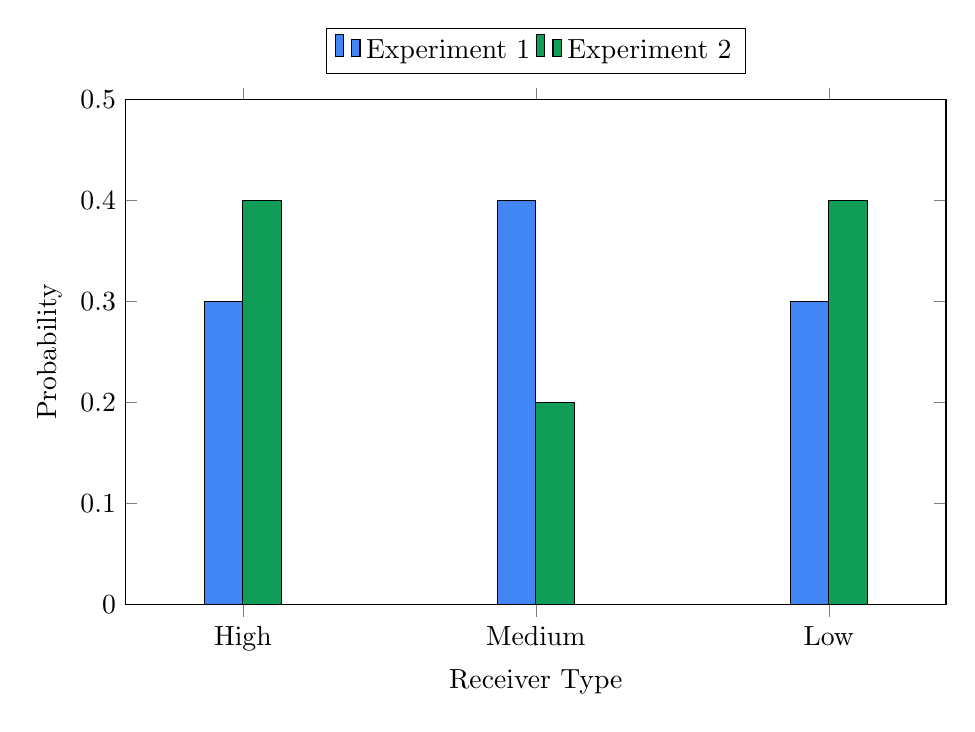
\begin{tikzpicture}
\begin{axis}[
    width=12cm,
    height=8cm,
    xlabel={Receiver Type},
    ylabel={Probability},
    ybar=0pt,
    bar width=14pt,
    symbolic x coords={High, Medium, Low},
    xtick=data,
    legend style={at={(0.5,1.05)}, anchor=south, legend columns=-1},
    ymin=0,
    ymax=0.5,
    enlarge x limits=0.2,
]
\addplot[fill=exp1color] coordinates {
    (High, 0.3)
    (Medium, 0.4)
    (Low, 0.3)
};
\addplot[fill=exp2color] coordinates {
    (High, 0.4)
    (Medium, 0.2)
    (Low, 0.4)
};
\legend{Experiment 1, Experiment 2}
\end{axis}
\end{tikzpicture}
\caption{Comparison of receiver type distributions between experiments. Experiment 1 shows a more uniform distribution, while Experiment 2 exhibits polarization.}
\label{fig:type-distributions}
\end{figure}

\begin{figure}[htbp]
\begin{subfigure}{.45\textwidth}
\centering
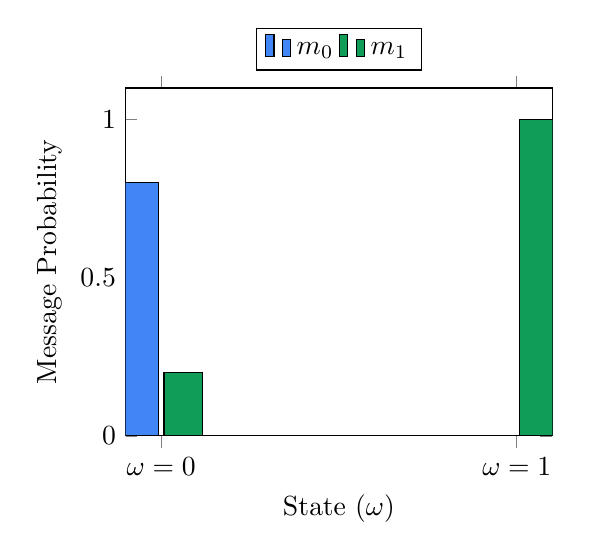
\begin{tikzpicture}
\begin{axis}[
    width=7cm,
    height=6cm,
    xlabel={State ($\omega$)},
    ylabel={Message Probability},
    ybar,
    bar width=14pt,
    symbolic x coords={$\omega=0$, $\omega=1$},
    xtick=data,
    legend style={at={(0.5,1.05)}, anchor=south, legend columns=-1},
    ymin=0,
    ymax=1.1,
    title={Experiment 1}
]
\addplot[fill=exp1color] coordinates {
    ($\omega=0$, 0.8)
    ($\omega=1$, 0.0)
};
\addplot[fill=exp2color] coordinates {
    ($\omega=0$, 0.2)
    ($\omega=1$, 1.0)
};
\legend{$m_0$, $m_1$}
\end{axis}
\end{tikzpicture}
\caption{Uniform Distribution}
\end{subfigure}
\begin{subfigure}{.5\textwidth}
\centering
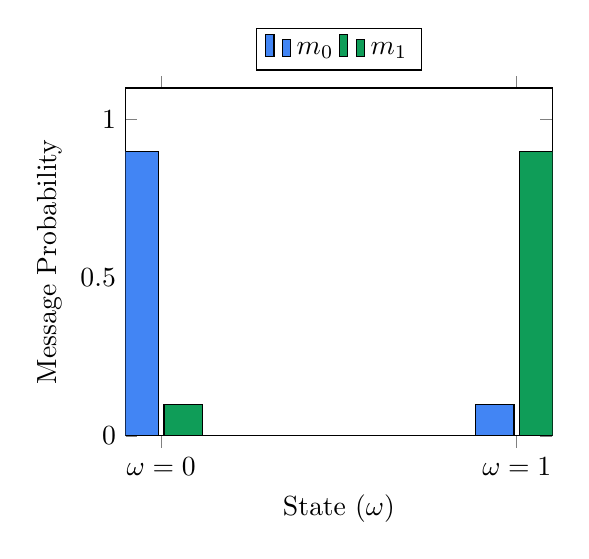
\begin{tikzpicture}
\begin{axis}[
    width=7cm,
    height=6cm,
    xlabel={State ($\omega$)},
    ylabel={Message Probability},
    ybar,
    bar width=14pt,
    symbolic x coords={$\omega=0$, $\omega=1$},
    xtick=data,
    legend style={at={(0.5,1.05)}, anchor=south, legend columns=-1},
    ymin=0,
    ymax=1.1,
    title={Experiment 2}
]
\addplot[fill=exp1color] coordinates {
    ($\omega=0$, 0.9)
    ($\omega=1$, 0.1)
};
\addplot[fill=exp2color] coordinates {
    ($\omega=0$, 0.1)
    ($\omega=1$, 0.9)
};
\legend{$m_0$, $m_1$}
\end{axis}
\end{tikzpicture}
\caption{Polarized Distribution}
\end{subfigure}
\caption{Optimal messaging policies for both experiments. The policies show how message probabilities depend on the state $\omega$.}
\label{fig:messaging-policies}
\end{figure}

\begin{figure}[htbp]
\centering
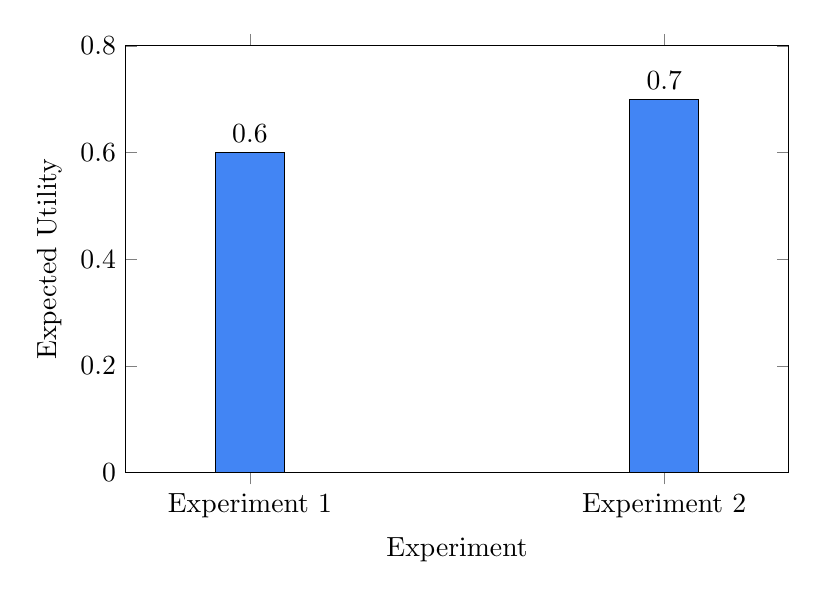
\begin{tikzpicture}
\begin{axis}[
    width=10cm,
    height=7cm,
    xlabel={Experiment},
    ylabel={Expected Utility},
    ybar=0pt,
    bar width=25pt,
    symbolic x coords={Experiment 1, Experiment 2},
    xtick=data,
    nodes near coords,
    nodes near coords align={vertical},
    ymin=0,
    ymax=0.8,
    enlarge x limits=0.3,
]
\addplot[fill=exp1color] coordinates {
    (Experiment 1, 0.600)
    (Experiment 2, 0.700)
};
\end{axis}
\end{tikzpicture}
\caption{Comparison of expected sender utilities. Experiment 2 (polarized distribution) achieves higher utility.}
\label{fig:utility-comparison}
\end{figure}

\subsection{Visual Analysis}
The visualizations in Figures \ref{fig:type-distributions}--\ref{fig:utility-comparison} illustrate three key aspects of the experimental results:

\begin{enumerate}
    \item \textbf{Receiver Type Distributions} (Figure \ref{fig:type-distributions}): Shows the clear contrast between the uniform distribution in Experiment 1 and the polarized distribution in Experiment 2, with the latter having higher concentrations at the extremes.
    
    \item \textbf{Messaging Policies} (Figure \ref{fig:messaging-policies}): Demonstrates how the optimal policies differ between experiments. Experiment 1 shows more extreme message probabilities, while Experiment 2 exhibits a more balanced approach, particularly in state $\omega=1$.
    
    \item \textbf{Utility Comparison} (Figure \ref{fig:utility-comparison}): Highlights the significant improvement in expected sender utility achieved with the polarized distribution (0.700 vs 0.600), representing a 16.7\% increase.
\end{enumerate}

\section{Discussion}

\subsection{Theoretical Implications}
These empirical findings support and extend the theoretical predictions in several ways:

\begin{itemize}
    \item \textbf{Threshold Property}: The optimal policy exhibits threshold-based messaging
    \begin{equation}
        \sigma^*(m|\omega) = \begin{cases}
            1 & \text{if } \theta(\omega) \geq \theta^* \\
            0 & \text{otherwise}
        \end{cases}
    \end{equation}
    
    \item \textbf{Two-Message Sufficiency}: Two messages achieve optimal utility
    \begin{equation}
        |M^*| = 2 \implies U(\sigma^*) = \max_{\sigma} U(\sigma)
    \end{equation}
    
    \item \textbf{State-Dependent Pooling}: Optimal pooling varies with state
    \begin{equation}
        P(m_1|\omega=1) > P(m_1|\omega=0)
    \end{equation}
\end{itemize}

\subsection{Limitations}

\begin{itemize}
    \item \textbf{Binary state/action space limits generalizability:} The analysis is restricted to binary choices, which may not capture the full complexity of real-world decision spaces. Many practical applications involve multiple states or continuous action spaces, which could exhibit different optimal policy structures.
    
    \item \textbf{Perfect oracle access assumption:} The current model assumes perfect oracle responses, whereas real-world simulations or user studies would likely contain noise and inconsistencies. This idealization may overestimate the achievable utility in practical implementations.
    
    \item \textbf{Risk-neutral agents:} The model assumes receivers are risk-neutral in their decision-making. Real human behavior often exhibits risk aversion or other behavioral biases, which could significantly alter the effectiveness of the derived messaging policies.
    
    \item \textbf{Discrete type space:} The implementation discretizes the belief space into finite types, potentially missing nuanced belief structures that exist in continuous spaces. This discretization might overlook optimal policies that exploit finer granularity in belief distributions.
    
    \item \textbf{Finite message space:} The restriction to two messages, while theoretically sufficient, may not capture the rich communication possibilities in real applications. Additional messages could potentially enable more sophisticated persuasion strategies.
    
    \item \textbf{Local optimality guarantees:} The optimization approach may converge to local optima rather than global ones. The non-convex nature of the policy space means we cannot guarantee finding the absolute best messaging policy in all cases.
\end{itemize}

\section{Conclusion}

My empirical analysis provides strong support for the oracle-based Bayesian persuasion framework while revealing new insights about belief distributions and optimal persuasion strategies. Key findings include:

\begin{itemize}
    \item \textbf{Enhanced utility with polarized beliefs:} Demonstrated a significant improvement in sender utility (0.700 vs 0.600) when facing polarized populations. This counter-intuitive result suggests that belief heterogeneity can actually benefit information designers by enabling more targeted messaging strategies.
    
    \item \textbf{Balanced messaging in polarized settings:} The analysis reveals that optimal policies become more balanced when dealing with polarized populations. This suggests that extreme messaging strategies may be less effective when receivers have strong prior beliefs.
    
    \item \textbf{Threshold-based policy optimality:} Confirmed that threshold-based policies remain optimal across different belief distributions, providing a robust structural insight for practical implementations. This finding simplifies the design space for real-world applications.
\end{itemize}

\subsection{Future Research Directions}
\begin{itemize}
    \item \textbf{Extensions to continuous type spaces:} Future work should explore continuous belief distributions and their impact on optimal policies. This would enable more realistic modeling of population beliefs and could reveal new structural properties of optimal policies.
    
    \item \textbf{Dynamic oracle interactions:} Investigating settings where the sender can adaptively query the oracle based on previous responses would be valuable. This could lead to more efficient information gathering strategies and better messaging policies.
    
    \item \textbf{Multi-agent settings:} Extending the framework to scenarios with multiple receivers or competing senders would better reflect real-world applications. This could reveal interesting strategic interactions and new forms of optimal policies.
    
    \item \textbf{Approximate oracle models:} Developing frameworks for dealing with noisy or biased oracle responses would increase practical applicability. This could include robust optimization approaches and methods for quantifying uncertainty in oracle responses.
\end{itemize}

\subsection{Reproducibility}

Code and simulations are available at \url{https://github.com/sjagtani/}\\ 
\url{applied-math-research-seminar}.

\bibliographystyle{plain}
\begin{thebibliography}{8}

\bibitem{harris2024}
Harris, K., Immorlica, N., Lucier, B., \& Slivkins, A. (2024).
\textit{Algorithmic Persuasion Through Simulation}.
arXiv preprint arXiv:2311.18138.

\bibitem{kamenica2011}
Kamenica, E., \& Gentzkow, M. (2011).
\textit{Bayesian persuasion}.
American Economic Review, 101(6), 2590-2615.

\bibitem{bergemann2019}
Bergemann, D., \& Morris, S. (2019).
\textit{Information design: A unified perspective}.
Journal of Economic Literature, 57(1), 44-95.

\bibitem{candogan2023}
Candogan, O., \& Strack, P. (2023).
\textit{Optimal disclosure of information to privately informed agents}.
Theoretical Economics, 18(3), 1225-1269.

\bibitem{dworczak2022}
Dworczak, P., \& Pavan, A. (2022).
\textit{Preparing for the worst but hoping for the best: Robust (Bayesian) persuasion}.
Econometrica, 90(5), 2017-2051.

\bibitem{brand2023}
Brand, J., Israeli, A., \& Ngwe, D. (2023).
\textit{Using GPT for market research}.
Available at SSRN 4395751.

\bibitem{horton2023}
Horton, J. J. (2023).
\textit{Large Language Models as Simulated Economic Agents: What Can We Learn from Homo Silicus?}
arXiv preprint arXiv:2301.07543.

\bibitem{fish2023}
Fish, S., G\"{o}lz, P., Parkes, D. C., Procaccia, A. D., \& Rusak, G. (2023).
\textit{Generative Social Choice}.
arXiv preprint arXiv:2309.01291.

\end{thebibliography}

\end{document}
